% Options for packages loaded elsewhere
\PassOptionsToPackage{unicode}{hyperref}
\PassOptionsToPackage{hyphens}{url}
\PassOptionsToPackage{dvipsnames,svgnames*,x11names*}{xcolor}
%
\documentclass[
  ignorenonframetext,
  aspectratio=169,
  serif,onlymath]{beamer}
\usepackage{pgfpages}
\setbeamertemplate{caption}[numbered]
\setbeamertemplate{caption label separator}{: }
\setbeamercolor{caption name}{fg=normal text.fg}
\beamertemplatenavigationsymbolsempty
% Prevent slide breaks in the middle of a paragraph
\widowpenalties 1 10000
\raggedbottom
\setbeamertemplate{part page}{
  \centering
  \begin{beamercolorbox}[sep=16pt,center]{part title}
    \usebeamerfont{part title}\insertpart\par
  \end{beamercolorbox}
}
\setbeamertemplate{section page}{
  \centering
  \begin{beamercolorbox}[sep=12pt,center]{part title}
    \usebeamerfont{section title}\insertsection\par
  \end{beamercolorbox}
}
\setbeamertemplate{subsection page}{
  \centering
  \begin{beamercolorbox}[sep=8pt,center]{part title}
    \usebeamerfont{subsection title}\insertsubsection\par
  \end{beamercolorbox}
}
\AtBeginPart{
  \frame{\partpage}
}
\AtBeginSection{
  \ifbibliography
  \else
    \frame{\sectionpage}
  \fi
}
\AtBeginSubsection{
  \frame{\subsectionpage}
}
\usepackage{lmodern}
\usepackage{amssymb,amsmath}
\usepackage{ifxetex,ifluatex}
\ifnum 0\ifxetex 1\fi\ifluatex 1\fi=0 % if pdftex
  \usepackage[T1]{fontenc}
  \usepackage[utf8]{inputenc}
  \usepackage{textcomp} % provide euro and other symbols
\else % if luatex or xetex
  \usepackage{unicode-math}
  \defaultfontfeatures{Scale=MatchLowercase}
  \defaultfontfeatures[\rmfamily]{Ligatures=TeX,Scale=1}
\fi
% Use upquote if available, for straight quotes in verbatim environments
\IfFileExists{upquote.sty}{\usepackage{upquote}}{}
\IfFileExists{microtype.sty}{% use microtype if available
  \usepackage[]{microtype}
  \UseMicrotypeSet[protrusion]{basicmath} % disable protrusion for tt fonts
}{}
\makeatletter
\@ifundefined{KOMAClassName}{% if non-KOMA class
  \IfFileExists{parskip.sty}{%
    \usepackage{parskip}
  }{% else
    \setlength{\parindent}{0pt}
    \setlength{\parskip}{6pt plus 2pt minus 1pt}}
}{% if KOMA class
  \KOMAoptions{parskip=half}}
\makeatother
\usepackage{xcolor}
\IfFileExists{xurl.sty}{\usepackage{xurl}}{} % add URL line breaks if available
\IfFileExists{bookmark.sty}{\usepackage{bookmark}}{\usepackage{hyperref}}
\hypersetup{
  pdftitle={Ellipsoid Method and the Amazing Oracles (I)},
  pdfauthor={Wai-Shing Luk},
  colorlinks=true,
  linkcolor=Maroon,
  filecolor=Maroon,
  citecolor=Blue,
  urlcolor=Blue,
  pdfcreator={LaTeX via pandoc}}
\urlstyle{same} % disable monospaced font for URLs
\newif\ifbibliography
\usepackage{color}
\usepackage{fancyvrb}
\newcommand{\VerbBar}{|}
\newcommand{\VERB}{\Verb[commandchars=\\\{\}]}
\DefineVerbatimEnvironment{Highlighting}{Verbatim}{commandchars=\\\{\}}
% Add ',fontsize=\small' for more characters per line
\newenvironment{Shaded}{}{}
\newcommand{\AlertTok}[1]{\textcolor[rgb]{1.00,0.00,0.00}{\textbf{#1}}}
\newcommand{\AnnotationTok}[1]{\textcolor[rgb]{0.38,0.63,0.69}{\textbf{\textit{#1}}}}
\newcommand{\AttributeTok}[1]{\textcolor[rgb]{0.49,0.56,0.16}{#1}}
\newcommand{\BaseNTok}[1]{\textcolor[rgb]{0.25,0.63,0.44}{#1}}
\newcommand{\BuiltInTok}[1]{#1}
\newcommand{\CharTok}[1]{\textcolor[rgb]{0.25,0.44,0.63}{#1}}
\newcommand{\CommentTok}[1]{\textcolor[rgb]{0.38,0.63,0.69}{\textit{#1}}}
\newcommand{\CommentVarTok}[1]{\textcolor[rgb]{0.38,0.63,0.69}{\textbf{\textit{#1}}}}
\newcommand{\ConstantTok}[1]{\textcolor[rgb]{0.53,0.00,0.00}{#1}}
\newcommand{\ControlFlowTok}[1]{\textcolor[rgb]{0.00,0.44,0.13}{\textbf{#1}}}
\newcommand{\DataTypeTok}[1]{\textcolor[rgb]{0.56,0.13,0.00}{#1}}
\newcommand{\DecValTok}[1]{\textcolor[rgb]{0.25,0.63,0.44}{#1}}
\newcommand{\DocumentationTok}[1]{\textcolor[rgb]{0.73,0.13,0.13}{\textit{#1}}}
\newcommand{\ErrorTok}[1]{\textcolor[rgb]{1.00,0.00,0.00}{\textbf{#1}}}
\newcommand{\ExtensionTok}[1]{#1}
\newcommand{\FloatTok}[1]{\textcolor[rgb]{0.25,0.63,0.44}{#1}}
\newcommand{\FunctionTok}[1]{\textcolor[rgb]{0.02,0.16,0.49}{#1}}
\newcommand{\ImportTok}[1]{#1}
\newcommand{\InformationTok}[1]{\textcolor[rgb]{0.38,0.63,0.69}{\textbf{\textit{#1}}}}
\newcommand{\KeywordTok}[1]{\textcolor[rgb]{0.00,0.44,0.13}{\textbf{#1}}}
\newcommand{\NormalTok}[1]{#1}
\newcommand{\OperatorTok}[1]{\textcolor[rgb]{0.40,0.40,0.40}{#1}}
\newcommand{\OtherTok}[1]{\textcolor[rgb]{0.00,0.44,0.13}{#1}}
\newcommand{\PreprocessorTok}[1]{\textcolor[rgb]{0.74,0.48,0.00}{#1}}
\newcommand{\RegionMarkerTok}[1]{#1}
\newcommand{\SpecialCharTok}[1]{\textcolor[rgb]{0.25,0.44,0.63}{#1}}
\newcommand{\SpecialStringTok}[1]{\textcolor[rgb]{0.73,0.40,0.53}{#1}}
\newcommand{\StringTok}[1]{\textcolor[rgb]{0.25,0.44,0.63}{#1}}
\newcommand{\VariableTok}[1]{\textcolor[rgb]{0.10,0.09,0.49}{#1}}
\newcommand{\VerbatimStringTok}[1]{\textcolor[rgb]{0.25,0.44,0.63}{#1}}
\newcommand{\WarningTok}[1]{\textcolor[rgb]{0.38,0.63,0.69}{\textbf{\textit{#1}}}}
\usepackage{graphicx,grffile}
\makeatletter
\def\maxwidth{\ifdim\Gin@nat@width>\linewidth\linewidth\else\Gin@nat@width\fi}
\def\maxheight{\ifdim\Gin@nat@height>\textheight\textheight\else\Gin@nat@height\fi}
\makeatother
% Scale images if necessary, so that they will not overflow the page
% margins by default, and it is still possible to overwrite the defaults
% using explicit options in \includegraphics[width, height, ...]{}
\setkeys{Gin}{width=\maxwidth,height=\maxheight,keepaspectratio}
% Set default figure placement to htbp
\makeatletter
\def\fps@figure{htbp}
\makeatother
\setlength{\emergencystretch}{3em} % prevent overfull lines
\providecommand{\tightlist}{%
  \setlength{\itemsep}{0pt}\setlength{\parskip}{0pt}}
\setcounter{secnumdepth}{-\maxdimen} % remove section numbering
\usetheme{default}
\usepackage{tikz,pgf,pgfplots}
\usetikzlibrary{arrows}
\definecolor{qqqqff}{rgb}{0.,0.,1.}
\newcommand{\columnsbegin}{\begin{columns}}
\newcommand{\columnsend}{\end{columns}}
\newcommand{\col}[1]{\column{#1}}
\pgfdeclareimage[height=0.5cm]{fudan-logo}{fudan-logo.jpg}
\logo{\pgfuseimage{fudan-logo}}
\makeatletter
\@ifpackageloaded{subfig}{}{\usepackage{subfig}}
\@ifpackageloaded{caption}{}{\usepackage{caption}}
\captionsetup[subfloat]{margin=0.5em}
\AtBeginDocument{%
\renewcommand*\figurename{Figure}
\renewcommand*\tablename{Table}
}
\AtBeginDocument{%
\renewcommand*\listfigurename{List of Figures}
\renewcommand*\listtablename{List of Tables}
}
\@ifpackageloaded{float}{}{\usepackage{float}}
\floatstyle{ruled}
\@ifundefined{c@chapter}{\newfloat{codelisting}{h}{lop}}{\newfloat{codelisting}{h}{lop}[chapter]}
\floatname{codelisting}{Listing}
\newcommand*\listoflistings{\listof{codelisting}{List of Listings}}
\makeatother
\usepackage[]{natbib}
\bibliographystyle{plainnat}

\title{Ellipsoid Method and the Amazing Oracles (I)}
\author{Wai-Shing Luk}
\date{\today}
\institute{Fudan University}

\begin{document}
\frame{\titlepage}

\begin{frame}
  \tableofcontents[hideallsubsections]
\end{frame}
\hypertarget{introduction}{%
\section{Introduction}\label{introduction}}

\begin{frame}

\begin{quote}
When you have eliminated the impossible, whatever remains, however
improbable, must be the truth.
\end{quote}

\emph{Sir Arthur Conan Doyle, stated by Sherlock Holmes}

\end{frame}

\begin{frame}{Common Perspective of Ellipsoid Method}
\protect\hypertarget{common-perspective-of-ellipsoid-method}{}

\begin{itemize}
\item
  It is commonly believed that it is inefficient in practice for
  large-scale problems.

  \begin{itemize}
  \item
    The convergent rate is slow, even with the use of deep cuts.
  \item
    Cannot exploit sparsity.
  \end{itemize}
\item
  Since then, it was supplanted by interior-point methods.
\item
  Only treated as a theoretical tool for proving the polynomial-time
  solvability of combinatorial optimization problems.
\end{itemize}

\end{frame}

\begin{frame}{But\ldots{}}
\protect\hypertarget{but}{}

\begin{itemize}
\item
  The ellipsoid method works very differently compared with the interior
  point method.
\item
  Only require a \emph{separtion oracle}. Can play nicely with other
  techniques.
\item
  The ellipsoid method itself cannot exploit sparsity, but the oracle
  can.
\end{itemize}

\end{frame}

\begin{frame}{Consider Ellipsoid Method When\ldots{}}
\protect\hypertarget{consider-ellipsoid-method-when}{}

\begin{itemize}
\item
  The number of optimization variables is moderate, e.g.~ECO flow,
  analog circuit sizing, parametric problems
\item
  The number of constraints is large, or even infinite
\item
  Oracle can be implemented efficiently.
\end{itemize}

\end{frame}

\hypertarget{cutting-plane-method-revisited}{%
\section{Cutting-plane Method
Revisited}\label{cutting-plane-method-revisited}}

\begin{frame}{Basic Idea}
\protect\hypertarget{basic-idea}{}

\begin{columns}
\column{0.6\textwidth}

\begin{itemize}
\tightlist
\item
  Let \(\mathcal{K} \subseteq \mathbb{R}^n\) be a convex set.
\item
  Consider the feasibility problem:

  \begin{itemize}
  \tightlist
  \item
    Find a point \(x^* \in \mathbb{R}^n\) in \(\mathcal{K}\),
  \item
    or determine that \(\mathcal{K}\) is empty (i.e., no feasible
    solution)
  \end{itemize}
\end{itemize}

\column{0.4\textwidth}

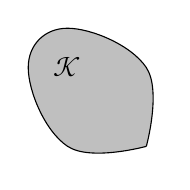
\begin{tikzpicture}[scale=0.5]
    \draw[top color=lightgray, bottom color=lightgray] plot[smooth, tension=.7] coordinates {(-3,2) (-5,2) (-6,4) (-5,5) (-3,4) (-3,2)};
    \node at (-5,4) {$\mathcal{K}$};
\end{tikzpicture}

\end{columns}

\end{frame}

\begin{frame}{Separation Oracle}
\protect\hypertarget{separation-oracle}{}

\begin{columns}
\column{0.6\textwidth}

\begin{itemize}
\tightlist
\item
  When a separation oracle \(\Omega\) is \emph{queried} at \(x_0\), it
  either

  \begin{itemize}
  \tightlist
  \item
    asserts that \(x_0 \in \mathcal{K}\), or
  \item
    returns a separating hyperplane between \(x_0\) and \(\mathcal{K}\):
    \[g^\mathsf{T} (x - x_0) + \beta \le 0, \beta \ge 0, g \neq 0, \;
          \forall x \in \mathcal{K}\]
  \end{itemize}
\end{itemize}

\column{0.4\textwidth}

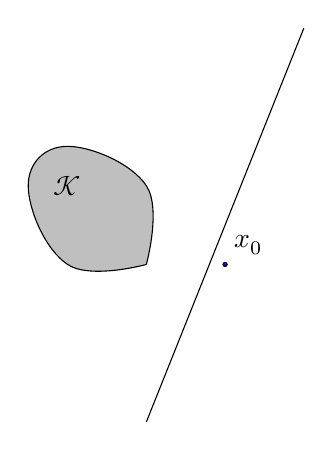
\begin{tikzpicture}[scale=0.5]
 \draw[top color=lightgray, bottom color=lightgray] plot[smooth, tension=.7] coordinates {(-3,2) (-5,2) (-6,4) (-5,5) (-3,4) (-3,2)};
 \node at (-5,4) {$\mathcal{K}$};
\draw (1,8) -- (-3,-2);
\draw [fill=qqqqff] (-1,2) circle (1.5pt)
   node [above right] {$x_0$};
\end{tikzpicture}

\end{columns}

\end{frame}

\begin{frame}{Separation oracle (cont'd)}
\protect\hypertarget{separation-oracle-contd}{}

\begin{itemize}
\item
  \((g, \beta)\) is called a \emph{cutting-plane}, or cut, since it
  eliminates the halfspace
  \(\{x \mid g^\mathsf{T} (x - x_0) + \beta > 0\}\) from our search.
\item
  If \(\beta=0\) (\(x_0\) is on the boundary of halfspace that is cut),
  cutting-plane is called \emph{neutral cut}.
\item
  If \(\beta>0\) (\(x_0\) lies in the interior of halfspace that is
  cut), cutting-plane is called \emph{deep cut}.
\item
  If \(\beta<0\) (\(x_0\) lies in the exterior of halfspace that is
  cut), cutting-plane is called \emph{shallow cut}.
\end{itemize}

\end{frame}

\begin{frame}{Subgradient}
\protect\hypertarget{subgradient}{}

\begin{itemize}
\item
  \(\mathcal{K}\) is usually given by a set of inequalities
  \(f_j(x) \le 0\) or \(f_j(x) < 0\) for \(j = 1 \cdots m\), where
  \(f_j(x)\) is a convex function.
\item
  A vector \(g \equiv \partial f(x_0)\) is called a subgradient of a
  convex function \(f\) at \(x_0\) if
  \(f(z) \ge f(x_0) + g^\mathsf{T} (z - x_0)\).
\item
  Hence, the cut \((g, \beta)\) is given by
  \((\partial f(x_0), f(x_0))\)
\end{itemize}

Remarks:

\begin{itemize}
\tightlist
\item
  If \(f(x)\) is differentiable, we can simply take
  \(\partial f(x_0) = \nabla f(x_0)\)
\end{itemize}

\end{frame}

\begin{frame}{Key components of Cutting-plane method}
\protect\hypertarget{key-components-of-cutting-plane-method}{}

\begin{itemize}
\tightlist
\item
  Cutting plane oracle \(\Omega\)
\item
  A search space \(\mathcal{S}\) initially big enough to cover
  \(\mathcal{K}\), e.g.

  \begin{itemize}
  \tightlist
  \item
    Polyhedron \(\mathcal{P}\) = \(\{z \mid C z \preceq d \}\)
  \item
    Interval \(\mathcal{I}\) = \([l, u]\) (for one-dimensional problem)
  \item
    Ellipsoid \(\mathcal{E}\) =
    \(\{z \mid (z-x_c)P^{-1}(z-x_c) \le 1 \}\)
  \end{itemize}
\end{itemize}

\end{frame}

\begin{frame}{Generic Cutting-plane method}
\protect\hypertarget{generic-cutting-plane-method}{}

\begin{itemize}
\tightlist
\item
  \textbf{Given} initial \(\mathcal{S}\) known to contain
  \(\mathcal{K}\).
\item
  \textbf{Repeat}

  \begin{enumerate}
  \tightlist
  \item
    Choose a point \(x_0\) in \(\mathcal{S}\)
  \item
    Query the cutting-plane oracle at \(x_0\)
  \item
    \textbf{If} \(x_0 \in \mathcal{K}\), quit
  \item
    \textbf{Else}, update \(\mathcal{S}\) to a smaller set that covers:
    \[\mathcal{S}^+ = \mathcal{S} \cap \{z \mid g^\mathsf{T} (z - x_0) + \beta \le 0\}\]
  \item
    \textbf{If} \(\mathcal{S}^+ = \emptyset\) or it is small enough,
    quit.
  \end{enumerate}
\end{itemize}

\end{frame}

\begin{frame}[fragile]{Corresponding Python code}
\protect\hypertarget{corresponding-python-code}{}

\scriptsize

\begin{Shaded}
\begin{Highlighting}[]
\KeywordTok{def}\NormalTok{ cutting_plane_feas(evaluate, S, options}\OperatorTok{=}\NormalTok{Options()):}
\NormalTok{    feasible }\OperatorTok{=} \VariableTok{False}
\NormalTok{    status }\OperatorTok{=} \DecValTok{0}
    \ControlFlowTok{for}\NormalTok{ niter }\KeywordTok{in} \BuiltInTok{range}\NormalTok{(options.max_it):}
\NormalTok{        cut, feasible }\OperatorTok{=}\NormalTok{ evaluate(S.xc)}
        \ControlFlowTok{if}\NormalTok{ feasible:  }\CommentTok{# feasible sol'n obtained}
            \ControlFlowTok{break}
\NormalTok{        status, tsq }\OperatorTok{=}\NormalTok{ S.update(cut)}
        \ControlFlowTok{if}\NormalTok{ status }\OperatorTok{!=} \DecValTok{0}\NormalTok{:  }\CommentTok{# empty cut}
            \ControlFlowTok{break}
        \ControlFlowTok{if}\NormalTok{ tsq }\OperatorTok{<}\NormalTok{ options.tol:}
\NormalTok{            status }\OperatorTok{=} \DecValTok{2}
            \ControlFlowTok{break}
    \ControlFlowTok{return}\NormalTok{ S.xc, niter}\OperatorTok{+}\DecValTok{1}\NormalTok{, feasible, status}
\end{Highlighting}
\end{Shaded}

\end{frame}

\begin{frame}{From Feasibility to Optimization}
\protect\hypertarget{from-feasibility-to-optimization}{}

\[\begin{array}{ll}
    \text{minimize}     & f_0(x), \\
    \text{subject to}   & x \in \mathcal{K}
\end{array}\]

\begin{itemize}
\item
  The optimization problem is treated as a feasibility problem with an
  additional constraint \(f_0(x) \le t\)
\item
  \(f_0(x)\) could be a convex function or a \emph{quasiconvex
  function}.
\item
  \(t\) is also called the \emph{best-so-far} value of \(f_0(x)\).
\end{itemize}

\end{frame}

\begin{frame}{Convex Optimization Problem}
\protect\hypertarget{convex-optimization-problem}{}

\begin{itemize}
\item
  Consider the following general form: \[\begin{array}{ll}
              \text{minimize}         & t, \\
              \text{subject to}   & \Phi(x, t) \le 0 \\
                                  & x \in \mathcal{K}
    \end{array}\] where \(\mathcal{K}'_t = \{x \mid \Phi(x, t) \le 0\}\)
  is the \(t\)-sublevel set of \(\{x \mid f_0(x) \le t\}\).
\item
  Note: \(\mathcal{K'}_t \subseteq \mathcal{K'}_u\) if and only if
  \(t \le u\) (monotonicity)
\item
  One easy way to solve the optimization problem is to apply the binary
  search on \(t\).
\end{itemize}

\end{frame}

\begin{frame}[fragile]

\scriptsize

\begin{Shaded}
\begin{Highlighting}[]
\KeywordTok{def}\NormalTok{ bsearch(evaluate, I, options}\OperatorTok{=}\NormalTok{Options()):}
\NormalTok{    feasible }\OperatorTok{=} \VariableTok{False}
\NormalTok{    l, u }\OperatorTok{=}\NormalTok{ I}
\NormalTok{    t }\OperatorTok{=}\NormalTok{ l }\OperatorTok{+}\NormalTok{ (u }\OperatorTok{-}\NormalTok{ l)}\OperatorTok{/}\DecValTok{2}
    \ControlFlowTok{for}\NormalTok{ niter }\KeywordTok{in} \BuiltInTok{range}\NormalTok{(options.max_it):}
        \ControlFlowTok{if}\NormalTok{ evaluate(t):  }\CommentTok{# feasible sol'n obtained}
\NormalTok{            feasible }\OperatorTok{=} \VariableTok{True}
\NormalTok{            u }\OperatorTok{=}\NormalTok{ t}
        \ControlFlowTok{else}\NormalTok{:}
\NormalTok{            l }\OperatorTok{=}\NormalTok{ t}
\NormalTok{        tau }\OperatorTok{=}\NormalTok{ (u }\OperatorTok{-}\NormalTok{ l)}\OperatorTok{/}\DecValTok{2}
\NormalTok{        t }\OperatorTok{=}\NormalTok{ l }\OperatorTok{+}\NormalTok{ tau}
        \ControlFlowTok{if}\NormalTok{ tau }\OperatorTok{<}\NormalTok{ options.tol:}
            \ControlFlowTok{break}
    \ControlFlowTok{return}\NormalTok{ u, niter}\OperatorTok{+}\DecValTok{1}\NormalTok{, feasible}
\end{Highlighting}
\end{Shaded}

\end{frame}

\begin{frame}[fragile]

\scriptsize

\begin{Shaded}
\begin{Highlighting}[]
\KeywordTok{class}\NormalTok{ bsearch_adaptor:}
    \KeywordTok{def} \FunctionTok{__init__}\NormalTok{(}\VariableTok{self}\NormalTok{, P, E, options}\OperatorTok{=}\NormalTok{Options()):}
        \VariableTok{self}\NormalTok{.P }\OperatorTok{=}\NormalTok{ P}
        \VariableTok{self}\NormalTok{.E }\OperatorTok{=}\NormalTok{ E}
        \VariableTok{self}\NormalTok{.options }\OperatorTok{=}\NormalTok{ options}

    \AttributeTok{@property}
    \KeywordTok{def}\NormalTok{ x_best(}\VariableTok{self}\NormalTok{):}
        \ControlFlowTok{return} \VariableTok{self}\NormalTok{.E.xc}

    \KeywordTok{def} \FunctionTok{__call__}\NormalTok{(}\VariableTok{self}\NormalTok{, t):}
\NormalTok{        E }\OperatorTok{=} \VariableTok{self}\NormalTok{.E.copy()}
        \VariableTok{self}\NormalTok{.P.update(t)}
\NormalTok{        x, _, feasible, _ }\OperatorTok{=}\NormalTok{ cutting_plane_feas(}
            \VariableTok{self}\NormalTok{.P, E, }\VariableTok{self}\NormalTok{.options)}
        \ControlFlowTok{if}\NormalTok{ feasible:}
            \VariableTok{self}\NormalTok{.E._xc }\OperatorTok{=}\NormalTok{ x.copy()}
            \ControlFlowTok{return} \VariableTok{True}
        \ControlFlowTok{return} \VariableTok{False}
\end{Highlighting}
\end{Shaded}

\end{frame}

\begin{frame}{Shrinking}
\protect\hypertarget{shrinking}{}

\begin{itemize}
\item
  Another possible way is, to update the best-so-far \(t\) whenever a
  feasible solution \(x_0\) is found by solving the equation
  \(\Phi(x_0, t_\text{new}) = 0\).
\item
  If the equation is difficuit to solve but \(t\) is also convex w.r.t.
  \(\Phi\), then we may create a new varaible, say \(x_{n+1}\) and let
  \(x_{n+1} \le t'\).
\end{itemize}

\end{frame}

\begin{frame}{Generic Cutting-plane method (Optim)}
\protect\hypertarget{generic-cutting-plane-method-optim}{}

\begin{itemize}
\tightlist
\item
  \textbf{Given} initial \(\mathcal{S}\) known to contain
  \(\mathcal{K}_t\).
\item
  \textbf{Repeat}

  \begin{enumerate}
  \tightlist
  \item
    Choose a point \(x_0\) in \(\mathcal{S}\)
  \item
    Query the separation oracle at \(x_0\)
  \item
    \textbf{If} \(x_0 \in \mathcal{K}_t\), update \(t\) such that
    \(\Phi(x_0, t) = 0\).
  \item
    Update \(\mathcal{S}\) to a smaller set that covers:
    \[\mathcal{S}^+ = \mathcal{S} \cap \{z \mid g^\mathsf{T} (z - x_0) + \beta \le 0\} \]
  \item
    \textbf{If} \(\mathcal{S}^+ = \emptyset\) or it is small enough,
    quit.
  \end{enumerate}
\end{itemize}

\end{frame}

\begin{frame}[fragile]

\scriptsize

\begin{Shaded}
\begin{Highlighting}[]
\KeywordTok{def}\NormalTok{ cutting_plane_dc(evaluate, S, t, options}\OperatorTok{=}\NormalTok{Options()):}
\NormalTok{    feasible }\OperatorTok{=} \VariableTok{False}  \CommentTok{# no sol'n}
\NormalTok{    x_best }\OperatorTok{=}\NormalTok{ S.xc}
    \ControlFlowTok{for}\NormalTok{ niter }\KeywordTok{in} \BuiltInTok{range}\NormalTok{(options.max_it):}
\NormalTok{        cut, t1 }\OperatorTok{=}\NormalTok{ evaluate(S.xc, t)}
        \ControlFlowTok{if}\NormalTok{ t }\OperatorTok{!=}\NormalTok{ t1:  }\CommentTok{# best t obtained}
\NormalTok{            feasible }\OperatorTok{=} \VariableTok{True}
\NormalTok{            t }\OperatorTok{=}\NormalTok{ t1}
\NormalTok{            x_best }\OperatorTok{=}\NormalTok{ S.xc}
\NormalTok{        status, tau }\OperatorTok{=}\NormalTok{ S.update(cut)}
        \ControlFlowTok{if}\NormalTok{ status }\OperatorTok{!=} \DecValTok{0}\NormalTok{:  }\CommentTok{# empty cut}
            \ControlFlowTok{break}
        \ControlFlowTok{if}\NormalTok{ tau }\OperatorTok{<}\NormalTok{ options.tol:}
\NormalTok{            status }\OperatorTok{=} \DecValTok{2}
            \ControlFlowTok{break}
    \ControlFlowTok{return}\NormalTok{ x_best, t, niter}\OperatorTok{+}\DecValTok{1}\NormalTok{, feasible, status}
\end{Highlighting}
\end{Shaded}

\end{frame}

\begin{frame}{Example - Profit Maximization Problem}
\protect\hypertarget{example---profit-maximization-problem}{}

This example is taken from \citep{Aliabadi2013Robust}.

\[\begin{array}{ll}
   \text{maximize} & p(A x_1^\alpha x_2^\beta) - v_1 x_1 - v_2 x_2 \\
   \text{subject to}& x_1 \le k.
\end{array}\]

\begin{itemize}
\tightlist
\item
  \(p(A x_1^\alpha x_2^\beta)\) : Cobb-Douglas production function
\item
  \(p\): the market price per unit
\item
  \(A\): the scale of production
\item
  \(\alpha, \beta\): the output elasticities
\item
  \(x\): input quantity
\item
  \(v\): output price
\item
  \(k\): a given constant that restricts the quantity of \(x_1\)
\end{itemize}

\end{frame}

\begin{frame}{Example - Profit maximization (cont'd)}
\protect\hypertarget{example---profit-maximization-contd}{}

\begin{itemize}
\tightlist
\item
  The formulation is not in the convex form.
\item
  Rewrite the problem in the following form: \[\begin{array}{ll}
    \text{maximize} & t \\
    \text{subject to} & t  + v_1 x_1  + v_2 x_2 \le p A x_1^{\alpha} x_2^{\beta}\\
                  & x_1 \le k.
    \end{array}\]
\end{itemize}

\end{frame}

\begin{frame}{Profit maximization in Convex Form}
\protect\hypertarget{profit-maximization-in-convex-form}{}

\begin{itemize}
\item
  By taking the logarithm of each variable:

  \begin{itemize}
  \tightlist
  \item
    \(y_1 = \log x_1\), \(y_2 = \log x_2\).
  \end{itemize}
\item
  We have the problem in a convex form:
\end{itemize}

\[\begin{array}{ll}
    \text{max}  & t \\
    \text{s.t.} & \log(t + v_1 e^{y_1} + v_2 e^{y_2}) - (\alpha y_1 + \beta y_2) \le \log(pA) \\
                & y_1 \le \log k.
\end{array}\]

\end{frame}

\begin{frame}[fragile]

\scriptsize

\begin{Shaded}
\begin{Highlighting}[]
\KeywordTok{class}\NormalTok{ profit_oracle:}
    \KeywordTok{def} \FunctionTok{__init__}\NormalTok{(}\VariableTok{self}\NormalTok{, params, a, v):}
\NormalTok{        p, A, k }\OperatorTok{=}\NormalTok{ params}
        \VariableTok{self}\NormalTok{.log_pA }\OperatorTok{=}\NormalTok{ np.log(p }\OperatorTok{*}\NormalTok{ A)}
        \VariableTok{self}\NormalTok{.log_k }\OperatorTok{=}\NormalTok{ np.log(k)}
        \VariableTok{self}\NormalTok{.v }\OperatorTok{=}\NormalTok{ v}
        \VariableTok{self}\NormalTok{.a }\OperatorTok{=}\NormalTok{ a}

    \KeywordTok{def} \FunctionTok{__call__}\NormalTok{(}\VariableTok{self}\NormalTok{, y, t):}
\NormalTok{        fj }\OperatorTok{=}\NormalTok{ y[}\DecValTok{0}\NormalTok{] }\OperatorTok{-} \VariableTok{self}\NormalTok{.log_k  }\CommentTok{# constraint}
        \ControlFlowTok{if}\NormalTok{ fj }\OperatorTok{>} \FloatTok{0.}\NormalTok{:}
\NormalTok{            g }\OperatorTok{=}\NormalTok{ np.array([}\FloatTok{1.}\NormalTok{, }\FloatTok{0.}\NormalTok{])}
            \ControlFlowTok{return}\NormalTok{ (g, fj), t}
\NormalTok{        log_Cobb }\OperatorTok{=} \VariableTok{self}\NormalTok{.log_pA }\OperatorTok{+}\NormalTok{ np.dot(}\VariableTok{self}\NormalTok{.a, y)}
\NormalTok{        x }\OperatorTok{=}\NormalTok{ np.exp(y)}
\NormalTok{        vx }\OperatorTok{=}\NormalTok{ np.dot(}\VariableTok{self}\NormalTok{.v, x)}
\NormalTok{        te }\OperatorTok{=}\NormalTok{ t }\OperatorTok{+}\NormalTok{ vx}
\NormalTok{        fj }\OperatorTok{=}\NormalTok{ np.log(te) }\OperatorTok{-}\NormalTok{ log_Cobb}
        \ControlFlowTok{if}\NormalTok{ fj }\OperatorTok{<} \FloatTok{0.}\NormalTok{:}
\NormalTok{            te }\OperatorTok{=}\NormalTok{ np.exp(log_Cobb)}
\NormalTok{            t }\OperatorTok{=}\NormalTok{ te }\OperatorTok{-}\NormalTok{ vx}
\NormalTok{            fj }\OperatorTok{=} \FloatTok{0.}
\NormalTok{        g }\OperatorTok{=}\NormalTok{ (}\VariableTok{self}\NormalTok{.v }\OperatorTok{*}\NormalTok{ x) }\OperatorTok{/}\NormalTok{ te }\OperatorTok{-} \VariableTok{self}\NormalTok{.a}
        \ControlFlowTok{return}\NormalTok{ (g, fj), t}
\end{Highlighting}
\end{Shaded}

\end{frame}

\begin{frame}[fragile]

\scriptsize

\begin{Shaded}
\begin{Highlighting}[]
\CommentTok{# Main program}

\ImportTok{import}\NormalTok{ numpy }\ImportTok{as}\NormalTok{ np}
\ImportTok{from}\NormalTok{ profit_oracle }\ImportTok{import} \OperatorTok{*}
\ImportTok{from}\NormalTok{ cutting_plane }\ImportTok{import} \OperatorTok{*}
\ImportTok{from}\NormalTok{ ell }\ImportTok{import} \OperatorTok{*}

\NormalTok{p, A, k }\OperatorTok{=} \FloatTok{20.0}\NormalTok{, }\FloatTok{40.0}\NormalTok{, }\FloatTok{30.5}
\NormalTok{params }\OperatorTok{=}\NormalTok{ p, A, k}
\NormalTok{a }\OperatorTok{=}\NormalTok{ np.array([}\FloatTok{0.1}\NormalTok{, }\FloatTok{0.4}\NormalTok{])}
\NormalTok{v }\OperatorTok{=}\NormalTok{ np.array([}\FloatTok{10.0}\NormalTok{, }\FloatTok{35.0}\NormalTok{])}
\NormalTok{y0 }\OperatorTok{=}\NormalTok{ np.array([}\FloatTok{0.}\NormalTok{, }\FloatTok{0.}\NormalTok{])  }\CommentTok{# initial x0}
\NormalTok{E }\OperatorTok{=}\NormalTok{ ell(}\DecValTok{200}\NormalTok{, y0)}
\NormalTok{P }\OperatorTok{=}\NormalTok{ profit_oracle(params, a, v)}
\NormalTok{yb1, fb, niter, feasible, status }\OperatorTok{=} \OperatorTok{\textbackslash{}}
\NormalTok{    cutting_plane_dc(P, E, }\FloatTok{0.0}\NormalTok{)}
\BuiltInTok{print}\NormalTok{(fb, niter, feasible, status)}
\end{Highlighting}
\end{Shaded}

\end{frame}

\begin{frame}{Area of Applications}
\protect\hypertarget{area-of-applications}{}

\begin{itemize}
\tightlist
\item
  Robust convex optimization

  \begin{itemize}
  \tightlist
  \item
    oracle technique: affine arithmetic
  \end{itemize}
\item
  Parametric network potential problem

  \begin{itemize}
  \tightlist
  \item
    oracle technique: negative cycle detection
  \end{itemize}
\item
  Semidefinite programming

  \begin{itemize}
  \tightlist
  \item
    oracle technique: Cholesky or \(LDL^\mathsf{T}\) factorization
  \end{itemize}
\end{itemize}

\end{frame}

\hypertarget{robust-convex-optimization}{%
\section{Robust Convex Optimization}\label{robust-convex-optimization}}

\begin{frame}{Robust Optimization Formulation}
\protect\hypertarget{robust-optimization-formulation}{}

\begin{itemize}
\item
  Consider: \[\begin{array}{ll}
      \text{minimize}   & \sup_{q \in \mathbb Q} f_0(x,q) \\
      \text{subject to} & f_j(x,q) \le 0, \;
       \forall q \in {\mathbb Q}, \; j = 1,2,\cdots,m,
    \end{array}\] where \(q\) represents a set of varying parameters.
\item
  The problem can be reformulated as: \[\begin{array}{ll}
      \text{minimize}   & t \\
      \text{subject to} & \sup_{q \in \mathbb Q} f_0(x,q) \le t  \\
      & f_j(x,q) \le 0, \;
       \forall q \in {\mathbb Q}, \; j = 1,2,\cdots,m,
    \end{array}\]
\end{itemize}

\end{frame}

\begin{frame}{Example - Profit Maximization Problem (convex)}
\protect\hypertarget{example---profit-maximization-problem-convex}{}

\[\begin{array}{ll}
\text{max}  & t \\
\text{s.t.} & \log(t + \hat{v}_1 e^{y_1} + \hat{v}_2 e^{y_2}) - (\hat{\alpha} y_1 + \hat{\beta} y_2) \le \log(\hat{p}\,A)  \\
                  & y_1 \le \log \hat{k} ,
\end{array}\]

\begin{itemize}
\tightlist
\item
  Now assume that:

  \begin{itemize}
  \tightlist
  \item
    \(\hat{\alpha}\) and \(\hat{\beta}\) vary \(\bar{\alpha} \pm e_1\)
    and \(\bar{\beta} \pm e_2\) respectively.
  \item
    \(\hat{p}\), \(\hat{k}\), \(\hat{v}_1\), and \(\hat{v}_2\) all vary
    \(\pm e_3\).
  \end{itemize}
\end{itemize}

\end{frame}

\begin{frame}{Example - Profit Maximization Problem (oracle)}
\protect\hypertarget{example---profit-maximization-problem-oracle}{}

By detail analysis, the worst case happens when:

\begin{itemize}
\tightlist
\item
  \(p = \bar{p} - e_3\), \(k = \bar{k} - e_3\)
\item
  \(v_1 = \bar{v}_1 + e_3\), \(v_2 = \bar{v}_2 + e_3\),
\item
  if \(y_1 > 0\), \(\alpha = \bar{\alpha} - e_1\), else
  \(\alpha = \bar{\alpha} + e_1\)
\item
  if \(y_2 > 0\), \(\beta = \bar{\beta} - e_2\), else
  \(\beta = \bar{\beta} + e_2\)
\end{itemize}

\end{frame}

\begin{frame}[fragile]

\scriptsize

\begin{Shaded}
\begin{Highlighting}[]
\KeywordTok{class}\NormalTok{ profit_rb_oracle:}
    \KeywordTok{def} \FunctionTok{__init__}\NormalTok{(}\VariableTok{self}\NormalTok{, params, a, v, vparams):}
\NormalTok{        ui, e1, e2, e3 }\OperatorTok{=}\NormalTok{ vparams}
        \VariableTok{self}\NormalTok{.uie }\OperatorTok{=}\NormalTok{ [ui }\OperatorTok{*}\NormalTok{ e1, ui }\OperatorTok{*}\NormalTok{ e2]}
        \VariableTok{self}\NormalTok{.a }\OperatorTok{=}\NormalTok{ a}
\NormalTok{        p, A, k }\OperatorTok{=}\NormalTok{ params}
\NormalTok{        p }\OperatorTok{-=}\NormalTok{ ui }\OperatorTok{*}\NormalTok{ e3}
\NormalTok{        k }\OperatorTok{-=}\NormalTok{ ui }\OperatorTok{*}\NormalTok{ e3}
\NormalTok{        v_rb }\OperatorTok{=}\NormalTok{ v.copy()}
\NormalTok{        v_rb }\OperatorTok{+=}\NormalTok{ ui }\OperatorTok{*}\NormalTok{ e3}
        \VariableTok{self}\NormalTok{.P }\OperatorTok{=}\NormalTok{ profit_oracle((p, A, k), a, v_rb)}

    \KeywordTok{def} \FunctionTok{__call__}\NormalTok{(}\VariableTok{self}\NormalTok{, y, t):}
\NormalTok{        a_rb }\OperatorTok{=} \VariableTok{self}\NormalTok{.a.copy()}
        \ControlFlowTok{for}\NormalTok{ i }\KeywordTok{in}\NormalTok{ [}\DecValTok{0}\NormalTok{, }\DecValTok{1}\NormalTok{]:}
\NormalTok{            a_rb[i] }\OperatorTok{+=} \VariableTok{self}\NormalTok{.uie[i] }\ControlFlowTok{if}\NormalTok{ y[i] }\OperatorTok{<=} \FloatTok{0.} \OperatorTok{\textbackslash{}}
                              \ControlFlowTok{else} \OperatorTok{-}\VariableTok{self}\NormalTok{.uie[i]}
        \VariableTok{self}\NormalTok{.P.a }\OperatorTok{=}\NormalTok{ a_rb}
        \ControlFlowTok{return} \VariableTok{self}\NormalTok{.P(y, t)}
\end{Highlighting}
\end{Shaded}

\end{frame}

\begin{frame}{Oracle in Robust Optimization Formulation}
\protect\hypertarget{oracle-in-robust-optimization-formulation}{}

\begin{itemize}
\tightlist
\item
  The oracle only needs to determine:

  \begin{itemize}
  \tightlist
  \item
    If \(f_j(x_0, q) > 0\) for some \(j\) and \(q = q_0\), then

    \begin{itemize}
    \tightlist
    \item
      the cut \((g, \beta)\) =
      \((\partial f_j(x_0, q_0), f_j(x_0, q_0))\)
    \end{itemize}
  \item
    If \(f_0(x_0, q) \ge t\) for some \(q = q_0\), then

    \begin{itemize}
    \tightlist
    \item
      the cut \((g, \beta)\) =
      \((\partial f_0(x_0, q_0), f_0(x_0, q_0) - t)\)
    \end{itemize}
  \item
    Otherwise, \(x_0\) is feasible, then

    \begin{itemize}
    \tightlist
    \item
      Let \(q_{\max} = \text{argmax}_{q \in \mathbb Q} f_0(x_0, q)\).
    \item
      \(t := f_0(x_0, q_{\max})\).
    \item
      The cut \((g, \beta)\) = \((\partial f_0(x_0, q_{\max}), 0)\)
    \end{itemize}
  \end{itemize}
\end{itemize}

Remark:

\begin{itemize}
\tightlist
\item
  for more complicated problems, affine arithmetic could be used
  \citep{liu2007robust}.
\end{itemize}

\end{frame}

\hypertarget{multi-parameter-network-problem}{%
\section{Multi-parameter Network
Problem}\label{multi-parameter-network-problem}}

\begin{frame}{Parametric Network Problem}
\protect\hypertarget{parametric-network-problem}{}

Given a network represented by a directed graph \(G = (V, E)\).

Consider:

\[\begin{array}{ll}
    \text{find} & x, {\color{red}u} \\
    \text{subject to} & {\color{red}u_j} - {\color{red}u_i} \le h_{ij}(x), \; \forall (i, j) \in E ,
   \end{array}\]

\begin{itemize}
\item
  \(h_{ij}(x)\) is the concave function of edge \((i,j)\),
\item
  Assume: network is large but the number of parameters is small.
\end{itemize}

\end{frame}

\begin{frame}{Network Potential Problem (cont'd)}
\protect\hypertarget{network-potential-problem-contd}{}

Given \(x\), the problem has a feasible solution if and only if \(G\)
contains no negative cycle. Let \(\mathcal{C}\) be a set of all cycles
of \(G\).

\[\begin{array}{ll}
    \text{find} & x \\
    \text{subject to} & w_k(x) \ge 0, \forall C_k \in \mathcal{C} ,
\end{array}\]

\begin{itemize}
\item
  \(C_k\) is a cycle of \(G\)
\item
  \(w_k(x) = \sum_{ (i,j)\in C_k} h_{ij}(x)\).
\end{itemize}

\end{frame}

\begin{frame}{Negative Cycle Finding}
\protect\hypertarget{negative-cycle-finding}{}

There are lots of methods to detect negative cycles in a weighted
graph~\citep{cherkassky1999negative}, in which Tarjan's
algorithm~\citep{Tarjan1981negcycle} is one of the fastest algorithms in
practice \citep{alg:dasdan_mcr, cherkassky1999negative}.

\end{frame}

\begin{frame}{Oracle in Network Potential Problem}
\protect\hypertarget{oracle-in-network-potential-problem}{}

\begin{itemize}
\tightlist
\item
  The oracle only needs to determine:

  \begin{itemize}
  \tightlist
  \item
    If there exists a negative cycle \(C_k\) under \(x_0\), then

    \begin{itemize}
    \tightlist
    \item
      the cut \((g, \beta)\) = \((-\partial w_k(x_0), -w_k(x_0))\)
    \end{itemize}
  \item
    Otherwise, the shortest path solution gives the value of
    \({\color{red}u}\).
  \end{itemize}
\end{itemize}

\end{frame}

\begin{frame}[fragile]{Python Code}
\protect\hypertarget{python-code}{}

\scriptsize

\begin{Shaded}
\begin{Highlighting}[]
\KeywordTok{class}\NormalTok{ network_oracle:}
    \KeywordTok{def} \FunctionTok{__init__}\NormalTok{(}\VariableTok{self}\NormalTok{, G, f, p):}
        \VariableTok{self}\NormalTok{.G }\OperatorTok{=}\NormalTok{ G}
        \VariableTok{self}\NormalTok{.f }\OperatorTok{=}\NormalTok{ f}
        \VariableTok{self}\NormalTok{.p }\OperatorTok{=}\NormalTok{ p  }\CommentTok{# partial derivative of f w.r.t x}
        \VariableTok{self}\NormalTok{.S }\OperatorTok{=}\NormalTok{ negCycleFinder(G)}

    \KeywordTok{def} \FunctionTok{__call__}\NormalTok{(}\VariableTok{self}\NormalTok{, x):}
        \KeywordTok{def}\NormalTok{ get_weight(G, e):}
            \ControlFlowTok{return} \VariableTok{self}\NormalTok{.f(G, e, x)}

        \VariableTok{self}\NormalTok{.S.get_weight }\OperatorTok{=}\NormalTok{ get_weight}
\NormalTok{        C }\OperatorTok{=} \VariableTok{self}\NormalTok{.S.find_neg_cycle()}
        \ControlFlowTok{if}\NormalTok{ C }\KeywordTok{is} \VariableTok{None}\NormalTok{:}
            \ControlFlowTok{return} \VariableTok{None}\NormalTok{, }\DecValTok{1}
\NormalTok{        f }\OperatorTok{=} \OperatorTok{-}\BuiltInTok{sum}\NormalTok{(}\VariableTok{self}\NormalTok{.f(}\VariableTok{self}\NormalTok{.G, e, x) }\ControlFlowTok{for}\NormalTok{ e }\KeywordTok{in}\NormalTok{ C)}
\NormalTok{        g }\OperatorTok{=} \OperatorTok{-}\BuiltInTok{sum}\NormalTok{(}\VariableTok{self}\NormalTok{.p(}\VariableTok{self}\NormalTok{.G, e, x) }\ControlFlowTok{for}\NormalTok{ e }\KeywordTok{in}\NormalTok{ C)}
        \ControlFlowTok{return}\NormalTok{ (g, f), }\DecValTok{0}
\end{Highlighting}
\end{Shaded}

\end{frame}

\begin{frame}{Example - Optimal Matrix Scaling
\citep{orlin1985computing}}
\protect\hypertarget{example---optimal-matrix-scaling-orlin1985computing}{}

\begin{itemize}
\item
  Given a sparse matrix \(A = [a_{ij}] \in \mathbb{R}^{N\times N}\).
\item
  Find another matrix \(B = U A U^{-1}\) where \(U\) is a nonnegative
  diagonal matrix, such that the ratio of any two elements of \(B\) in
  absolute value is as close to 1 as possible.
\item
  Let \(U = \mathrm{diag}([u_1, u_2, \ldots, u_N])\). Under the
  min-max-ratio criterion, the problem can be formulated as:
\end{itemize}

\[\begin{array}{ll}
  \text{minimize}   &   \pi/\psi  \\
  \text{subject to} &   \psi \le u_i |a_{ij}| u_j^{-1} \le \pi, \; \forall a_{ij} \neq 0 , \\
                    &   \pi, \psi, u, \, \text{positive} \\
  \text{variables}  &   \pi, \psi, u \, .
  \end{array}\]

\end{frame}

\begin{frame}{Optimal Matrix Scaling (cont'd)}
\protect\hypertarget{optimal-matrix-scaling-contd}{}

By taking the logarithms of variables, the above problem can be
transformed into:

\[\begin{array}{ll}
  \text{minimize}   &   t \\
  \text{subject to} &   {\color{blue}\pi'} - {\color{blue}\psi'} \le t \\
                    &   {\color{red}u_i'} - {\color{red}u_j'}  \le {\color{blue}\pi'} - a_{ij}', \; \forall a_{ij} \neq 0 \,, \\
                    &   {\color{red}u_j'} - {\color{red}u_i'} \le a_{ij}' - {\color{blue}\psi'}, \; \forall a_{ij} \neq 0 \,, \\
  \text{variables}  &   {\color{blue}\pi'}, {\color{blue}\psi'}, {\color{red}u'} \, .
  \end{array}\]

where \(k'\) denotes \(\log( | k | )\) and
\(x = ({\color{blue}\pi'}, {\color{blue}\psi'} )^\mathsf{T}\).

\end{frame}

\begin{frame}[fragile]{Corresponding Python Code}
\protect\hypertarget{corresponding-python-code-1}{}

\scriptsize

\begin{Shaded}
\begin{Highlighting}[]
\KeywordTok{def}\NormalTok{ constr(G, e, x):}
\NormalTok{    u, v }\OperatorTok{=}\NormalTok{ e}
\NormalTok{    i_u }\OperatorTok{=}\NormalTok{ G.node_idx[u]}
\NormalTok{    i_v }\OperatorTok{=}\NormalTok{ G.node_idx[v]}
\NormalTok{    cost }\OperatorTok{=}\NormalTok{ G[u][v][}\StringTok{'cost'}\NormalTok{]}
    \ControlFlowTok{return}\NormalTok{ x[}\DecValTok{0}\NormalTok{] }\OperatorTok{-}\NormalTok{ cost }\ControlFlowTok{if}\NormalTok{ i_u }\OperatorTok{<=}\NormalTok{ i_v }\ControlFlowTok{else}\NormalTok{ cost }\OperatorTok{-}\NormalTok{ x[}\DecValTok{1}\NormalTok{]}

\KeywordTok{def}\NormalTok{ pconstr(G, e, x):}
\NormalTok{    u, v }\OperatorTok{=}\NormalTok{ e}
\NormalTok{    i_u }\OperatorTok{=}\NormalTok{ G.node_idx[u]}
\NormalTok{    i_v }\OperatorTok{=}\NormalTok{ G.node_idx[v]}
    \ControlFlowTok{return}\NormalTok{ np.array([}\FloatTok{1.}\NormalTok{,  }\FloatTok{0.}\NormalTok{] }\ControlFlowTok{if}\NormalTok{ i_u }\OperatorTok{<=}\NormalTok{ i_v }\ControlFlowTok{else}\NormalTok{ [}\FloatTok{0.}\NormalTok{, }\FloatTok{-1.}\NormalTok{])}

\KeywordTok{class}\NormalTok{ optscaling_oracle:}
    \KeywordTok{def} \FunctionTok{__init__}\NormalTok{(}\VariableTok{self}\NormalTok{, G):}
        \VariableTok{self}\NormalTok{.network }\OperatorTok{=}\NormalTok{ network_oracle(G, constr, pconstr)}

    \KeywordTok{def} \FunctionTok{__call__}\NormalTok{(}\VariableTok{self}\NormalTok{, x, t):}
\NormalTok{        cut, feasible }\OperatorTok{=} \VariableTok{self}\NormalTok{.network(x)}
        \ControlFlowTok{if} \KeywordTok{not}\NormalTok{ feasible: }\ControlFlowTok{return}\NormalTok{ cut, t}
\NormalTok{        s }\OperatorTok{=}\NormalTok{ x[}\DecValTok{0}\NormalTok{] }\OperatorTok{-}\NormalTok{ x[}\DecValTok{1}\NormalTok{]}
\NormalTok{        fj }\OperatorTok{=}\NormalTok{ s }\OperatorTok{-}\NormalTok{ t}
        \ControlFlowTok{if}\NormalTok{ fj }\OperatorTok{<} \FloatTok{0.}\NormalTok{:}
\NormalTok{            t }\OperatorTok{=}\NormalTok{ s}
\NormalTok{            fj }\OperatorTok{=} \FloatTok{0.}
        \ControlFlowTok{return}\NormalTok{ (np.array([}\FloatTok{1.}\NormalTok{, }\FloatTok{-1.}\NormalTok{]), fj), t}
\end{Highlighting}
\end{Shaded}

\end{frame}

\begin{frame}{Example - clock period \& yield-driven co-optimization}
\protect\hypertarget{example---clock-period-yield-driven-co-optimization}{}

\[\begin{array}{cll}
   \text{minimize} &T_\text{CP} / {\color{blue}\beta} \\
   \text{subject to} & u_i - u_j \le T_\text{CP} - F_{ij}^{-1}({\color{blue}\beta}), & \forall (i,j) \in E_s \,,\\
                     & u_j - u_i \le F_{ij}^{-1}(1 - {\color{blue}\beta}), & \forall (j,i) \in E_h \,, \\
                     & T_\text{CP} \ge 0, \, 0 \le {\color{blue}\beta} \le 1 \, , \\
    \text{variables} &T_\text{CP}, {\color{blue}\beta}, u.
   \end{array}\]

\begin{itemize}
\tightlist
\item
  Note that \(F_{ij}^{-1}(x)\) is not concave in general in \([0, 1]\).
\item
  Fortunately, we are most likely interested in optimizing circuits for
  high yield rather than the low one in practice.
\item
  Therefore, by imposing an additional constraint to \(\beta\), say
  \(\beta \ge 0.8\), the problem becomes convex.
\end{itemize}

\end{frame}

\begin{frame}{Example - clock period \& yield-driven co-optimization}
\protect\hypertarget{example---clock-period-yield-driven-co-optimization-1}{}

The problem can be reformulated as:

\[\begin{array}{cll}
   \text{minimize}   & t \\
   \text{subject to} & T_\text{CP} - {\color{blue}\beta} t \le 0\\
                     & u_i - u_j \le T_\text{CP} - F_{ij}^{-1}({\color{blue}\beta}), & \forall (i,j) \in E_s \,,\\
                     & u_j - u_i \le F_{ij}^{-1}(1 - {\color{blue}\beta}), & \forall (j,i) \in E_h \,, \\
                     & T_\text{CP} \ge 0, \, 0 \le {\color{blue}\beta} \le 1 \, , \\
    \text{variables} &T_\text{CP}, {\color{blue}\beta}, u.
   \end{array}\]

\end{frame}

\hypertarget{matrix-inequalities}{%
\section{Matrix Inequalities}\label{matrix-inequalities}}

\begin{frame}{Problems With Matrix Inequalities}
\protect\hypertarget{problems-with-matrix-inequalities}{}

Consider the following problem:

\[\begin{array}{ll}
    \text{find}    & x, \\
    \text{subject to}  & F(x) \succeq 0,
\end{array}\]

\begin{itemize}
\tightlist
\item
  \(F(x)\): a matrix-valued function
\item
  \(A \succeq 0\) denotes \(A\) is positive semidefinite.
\end{itemize}

\end{frame}

\begin{frame}{Problems With Matrix Inequalities}
\protect\hypertarget{problems-with-matrix-inequalities-1}{}

\begin{itemize}
\tightlist
\item
  Recall that a matrix \(A\) is positive semidefinite if and only if
  \(v^\mathsf{T} A v \ge 0\) for all \(v \in \mathbb{R}^N\).
\item
  The problem can be transformed into: \[\begin{array}{ll}
            \text{find}      & x, \\
            \text{subject to}    & v^\mathsf{T} F(x) v \ge 0, \; \forall v \in \mathbb{R}^N
    \end{array}\]
\item
  Consider \(v^\mathsf{T} F(x) v\) is concave for all
  \(v \in \mathbb{R}^N\) w. r. t. \(x\), then the above problem is a
  convex programming.
\item
  Reduce to \emph{semidefinite programming} if \(F(x)\) is linear w.r.t.
  \(x\), i.e., \(F(x) = F_0 + x_1 F_1 + \cdots + x_n F_n\)
\end{itemize}

\end{frame}

\begin{frame}{Oracle in Matrix Inequalities}
\protect\hypertarget{oracle-in-matrix-inequalities}{}

The oracle only needs to:

\begin{itemize}
\tightlist
\item
  Perform a \emph{row-based} LDLT factorization such that
  \(F(x_0) = L D L^\mathsf{T}\).
\item
  Let \(A_{:p,:p}\) denotes a submatrix
  \(A(1:p, 1:p) \in \mathbb{R}^{p\times p}\).
\item
  If the process fails at row \(p\),

  \begin{itemize}
  \tightlist
  \item
    there exists a vector
    \(e_p = (0, 0, \cdots, 0, 1)^\mathsf{T} \in \mathbb{R}^p\), such
    that

    \begin{itemize}
    \tightlist
    \item
      \(v = R_{:p,:p}^{-1} e_p\), and
    \item
      \(v^\mathsf{T} F_{:p,:p}(x_0) v < 0\).
    \end{itemize}
  \item
    The cut \((g, \beta)\) =
    \((-v^\mathsf{T} \partial F_{:p,:p}(x_0) v, -v^\mathsf{T} F_{:p,:p}(x_0) v)\)
  \end{itemize}
\end{itemize}

\end{frame}

\begin{frame}{Lazy evaluation}
\protect\hypertarget{lazy-evaluation}{}

\begin{itemize}
\item
  Don't construct the full matrix at each iteration!
\item
  Only O(\(p^3\)) per iteration, independent of \(N\)!
\end{itemize}

\end{frame}

\begin{frame}[fragile]

\scriptsize

\begin{Shaded}
\begin{Highlighting}[]
\KeywordTok{class}\NormalTok{ lmi_oracle:}
    \CommentTok{''' Oracle for LMI constraint F*x <= B '''}

    \KeywordTok{def} \FunctionTok{__init__}\NormalTok{(}\VariableTok{self}\NormalTok{, F, B):}
        \VariableTok{self}\NormalTok{.F }\OperatorTok{=}\NormalTok{ F}
        \VariableTok{self}\NormalTok{.F0 }\OperatorTok{=}\NormalTok{ B}
        \VariableTok{self}\NormalTok{.Q }\OperatorTok{=}\NormalTok{ chol_ext(}\BuiltInTok{len}\NormalTok{(}\VariableTok{self}\NormalTok{.F0))}

    \KeywordTok{def} \FunctionTok{__call__}\NormalTok{(}\VariableTok{self}\NormalTok{, x):}
\NormalTok{        n }\OperatorTok{=} \BuiltInTok{len}\NormalTok{(x)}

        \KeywordTok{def}\NormalTok{ getA(i, j):}
            \ControlFlowTok{return} \VariableTok{self}\NormalTok{.F0[i, j] }\OperatorTok{-} \BuiltInTok{sum}\NormalTok{(}
                \VariableTok{self}\NormalTok{.F[k][i, j] }\OperatorTok{*}\NormalTok{ x[k] }\ControlFlowTok{for}\NormalTok{ k }\KeywordTok{in} \BuiltInTok{range}\NormalTok{(n))}

        \VariableTok{self}\NormalTok{.Q.factor(getA)}
        \ControlFlowTok{if} \VariableTok{self}\NormalTok{.Q.is_spd():}
            \ControlFlowTok{return} \VariableTok{None}\NormalTok{, }\VariableTok{True}
\NormalTok{        v, ep }\OperatorTok{=} \VariableTok{self}\NormalTok{.Q.witness()}
\NormalTok{        g }\OperatorTok{=}\NormalTok{ np.array([}\VariableTok{self}\NormalTok{.Q.sym_quad(v, }\VariableTok{self}\NormalTok{.F[i])}
                      \ControlFlowTok{for}\NormalTok{ i }\KeywordTok{in} \BuiltInTok{range}\NormalTok{(n)])}
        \ControlFlowTok{return}\NormalTok{ (g, ep), }\VariableTok{False}
\end{Highlighting}
\end{Shaded}

\end{frame}

\begin{frame}[fragile]{Google Benchmark Comparison}
\protect\hypertarget{google-benchmark-comparison}{}

\begin{verbatim}
2: ----------------------------------------------------------
2: Benchmark                Time             CPU   Iterations
2: ----------------------------------------------------------
2: BM_LMI_Lazy         131235 ns       131245 ns         4447
2: BM_LMI_old          196694 ns       196708 ns         3548
2/4 Test #2: Bench_BM_lmi .....................   Passed    2.57 sec
\end{verbatim}

\end{frame}

\begin{frame}{Example - Matrix Norm Minimization}
\protect\hypertarget{example---matrix-norm-minimization}{}

\begin{itemize}
\tightlist
\item
  Let \(A(x) = A_0 + x_1 A_1 + \cdots + x_n A_n\)
\item
  Problem \(\min_x \| A(x) \|\) can be reformulated as
  \[\begin{array}{ll}
       \text{minimize}      & t, \\
       \text{subject to}    & \left(
   \begin{array}{cc}
    t\,I   & A(x) \\
    A^\mathsf{T}(x) & t\,I
   \end{array} \right) \succeq 0,
   \end{array}\]
\item
  Binary search on \(t\) can be used for this problem.
\end{itemize}

\end{frame}

\begin{frame}{Example - Estimation of Correlation Function}
\protect\hypertarget{example---estimation-of-correlation-function}{}

\[\begin{array}{ll}
   \min_{{\color{blue}\kappa}, p}   & \| \Sigma({\color{blue}p}) + {\color{blue}\kappa} I - Y \| \\
   \text{s. t.} & \Sigma({\color{blue}p}) \succcurlyeq 0,  {\color{blue}\kappa} \ge 0 \; .\\
 \end{array}\]

\begin{itemize}
\item
  Let \(\rho(h) = \sum_i^n {\color{blue}p}_i \Psi_i(h)\), where

  \begin{itemize}
  \tightlist
  \item
    \(p_i\)'s are the unknown coefficients to be fitted
  \item
    \(\Psi_i\)'s are a family of basis functions.
  \end{itemize}
\item
  The covariance matrix \(\Sigma({\color{blue}p})\) can be recast as:
  \[\Sigma({\color{blue}p}) = {\color{blue}p}_1 F_1 + \cdots + {\color{blue}p}_n F_n\]

  where \(\{F_k\}_{i,j} =\Psi_k( \| s_j - s_i \|_2)\)
\end{itemize}

\end{frame}

\begin{frame}{Experimental Result (I)}
\protect\hypertarget{experimental-result-i}{}

\begin{columns}
\column{0.5\textwidth}

\begin{figure}
\centering
\includegraphics{ellipsoid.files/iso050.pdf}
\caption{Data Sample (kern=0.5)}
\end{figure}

\column{0.5\textwidth}

\begin{figure}
\centering
\includegraphics{ellipsoid.files/result050.pdf}
\caption{Least Square Result}
\end{figure}

\end{columns}

\end{frame}

\begin{frame}{Experimental Result (II)}
\protect\hypertarget{experimental-result-ii}{}

\begin{columns}
\column{0.5\textwidth}

\begin{figure}
\centering
\includegraphics{ellipsoid.files/iso100.pdf}
\caption{Data Sample (kern=1.0)}
\end{figure}

\column{0.5\textwidth}

\begin{figure}
\centering
\includegraphics{ellipsoid.files/result100.pdf}
\caption{Least Square Result}
\end{figure}

\end{columns}

\end{frame}

\begin{frame}{Experimental Result (III)}
\protect\hypertarget{experimental-result-iii}{}

\begin{columns}
\column{0.5\textwidth}

\begin{figure}
\centering
\includegraphics{ellipsoid.files/iso200.pdf}
\caption{Data Sample (kern=2.0)}
\end{figure}

\column{0.5\textwidth}

\begin{figure}
\centering
\includegraphics{ellipsoid.files/result200.pdf}
\caption{Least Square Result}
\end{figure}

\end{columns}

\end{frame}

\renewcommand\refname{Reference}
\begin{frame}[allowframebreaks]{Reference}
  \bibliographytrue
  \bibliography{ellipsoid,fir-ref,Geostatistics,mpcss1,mpcss2}
\end{frame}

\end{document}
